  \documentclass[11pt, a4paper]{article}
  \usepackage[inner=1.5cm,outer=1.5cm,top=2.5cm,bottom=2.5cm]{geometry}

\pagestyle{empty}
\usepackage{graphicx}
\usepackage{setspace}
\usepackage{threeparttable}
\usepackage{fancyhdr, lastpage, bbding, pmboxdraw}
\usepackage[usenames,dvipsnames]{color}
\definecolor{darkblue}{rgb}{0,0,.6}
\definecolor{darkred}{rgb}{.7,0,0}
\definecolor{darkgreen}{rgb}{0,.6,0}
\definecolor{red}{rgb}{.98,0,0}
\usepackage[colorlinks,pagebackref,pdfusetitle,urlcolor=darkblue,citecolor=darkblue,linkcolor=darkred,bookmarksnumbered,plainpages=false]{hyperref}
\renewcommand{\thefootnote}{\fnsymbol{footnote}}

\pagestyle{fancyplain}
\fancyhf{}
\lhead{ \fancyplain{}{Vertebrate Biodiversity Lab- Lab Breakdown} }
%\chead{ \fancyplain{}{} }
\rhead{ \fancyplain{}{\today} }
%\rfoot{\fancyplain{}{page \thepage\ of \pageref{LastPage}}}
\fancyfoot[RO, LE] {page \thepage\ of \pageref{LastPage} }
\thispagestyle{plain}

%%%%%%%%%%%% LISTING %%%
\usepackage{listings}
\usepackage{caption}
\DeclareCaptionFont{white}{\color{white}}
\DeclareCaptionFormat{listing}{\colorbox{gray}{\parbox{\textwidth}{#1#2#3}}}
\captionsetup[lstlisting]{format=listing,labelfont=white,textfont=white}
\usepackage{verbatim} % used to display code
\usepackage{fancyvrb}
\usepackage{acronym}
\usepackage{amsthm}
\usepackage{arydshln} % dashed line in table
\VerbatimFootnotes % Required, otherwise verbatim does not work in footnotes!



\definecolor{OliveGreen}{cmyk}{0.64,0,0.95,0.40}
\definecolor{CadetBlue}{cmyk}{0.62,0.57,0.23,0}
\definecolor{lightlightgray}{gray}{0.93}



\lstset{
%language=bash,                          % Code langugage
basicstyle=\ttfamily,                   % Code font, Examples: \footnotesize, \ttfamily
keywordstyle=\color{OliveGreen},        % Keywords font ('*' = uppercase)
commentstyle=\color{gray},              % Comments font
numbers=left,                           % Line nums position
numberstyle=\tiny,                      % Line-numbers fonts
stepnumber=1,                           % Step between two line-numbers
numbersep=5pt,                          % How far are line-numbers from code
backgroundcolor=\color{lightlightgray}, % Choose background color
frame=none,                             % A frame around the code
tabsize=2,                              % Default tab size
captionpos=t,                           % Caption-position = bottom
breaklines=true,                        % Automatic line breaking?
breakatwhitespace=false,                % Automatic breaks only at whitespace?
showspaces=false,                       % Dont make spaces visible
showtabs=false,                         % Dont make tabls visible
columns=flexible,                       % Column format
morekeywords={__global__, __device__},  % CUDA specific keywords
}

\begin{document}

\pagestyle{fancyplain}
\fancyhf{}
\lhead{ \fancyplain{}{BIOL 4020 – Vertebrate Biodiversity - Field Notebook}}
%\chead{ \fancyplain{}{}}
\rhead{ \fancyplain{}{Fall 2020}}
%\rfoot{\fancyplain{}{page \thepage\ of \pageref{LastPage}}}
\fancyfoot[RO, LE] {page \thepage\ of \pageref{LastPage}}
\thispagestyle{plain}

\begin{center}
\begin{singlespace}
\rule{6in}{0.4pt}
\begin{minipage}[t]{.75\textwidth}
\begin{tabular}{llll}
\textbf{Field Trip 1:} & Student 1,  Student 2,  Student 3 \\ \textbf{Field Trip 2:} & Student 4,  Student 5,  Student 6 \\ \textbf{Field Trip 3:} & Student 7,  Student 8,  Student 9 \\ \textbf{Field Trip 4:} & Student 10, Student 11, Student 12
\end{tabular}
\end{minipage}
\rule{6in}{0.4pt}
\end{singlespace}
\end{center}
\vspace{.5cm}
\setlength{\unitlength}{1in}
\renewcommand{\arraystretch}{2}


\justify
\noindent{\large{\textbf{Field Notebook Overview:}}}\\ %\footnotemark
\begin{itemize}
\item{To fulfill a central purpose of this lab (helping you understand and appreciate vertebrate biodiversity), we will be taking trips to the field to observe vertebrate animals in their natural environments. In addition to the trips we take as a class, you are required to obtain additional hours on your own field ``expeditions.'' Central to field biology is keeping useful notes of what you observe. This section provides everything you need to include in your field notebook to receive full credit.}
\item{$*$ Due to the COVID-19 pandemic, we will not be taking entire lab sections to field sites via university transport. Instead, three students per section will be pre-assigned dates (see table at top of page) when they will ride to sites via university transport. All members within the vehicle are required to wear a face mask, and the windows will be down for the duration of the trip (no trip is longer than 30 minutes). Other students are welcome to join trips, but must take their personal vehicles. We will record video highlights of lab trips and post these on canvas. These video highlights may include taxa and natural history facts that can be included on your exams.}
\end{itemize}

\vskip.15in
\noindent{\large{\textbf{Assignment Requirements:}}} %\footnotemark
\begin{itemize}
\item{To receive full points, you must log 12 hours dedicated to in-field observations. These hours must be dedicated to searching for vertebrate animals, identifying the animals (taking a photo will help), and observing behavior. Field observation hours cannot be a secondary activity (i.e., the primary purpose of you going to a site must be to observe vertebrate animals)}.
\item{To receive full credit, each journal entry requires an appropriate heading and Detailed observations (see below)}
\item{It is recommended to use a weather-proof field journal, but any notebook the size of a paperback novel is adequate.}
\item{4 points will be deducted for each hour a student is short of the 12 total hours}
\item{Being physically present on lab trips counts toward the 12 hours}
\item{If you are uncomfortable or unable to log all needed hours, additional hours can be obtained by contributing to iNaturalist (but this must be approved beforehand by a TA)}
\end{itemize} 

\vskip.15in
\begin{singlespace}
\noindent{\large{\textbf{Journal Entry Requirements:}}}\\ %\footnotemark
\begin{itemize}
	\item{heading:}
	\begin{itemize}
		\item{Your name}
		\item{Date}
		\item{General location (locality name, County, State)}
		\item{Specify what the weather has been like over the last few days}
		\item{Number of people}
	\end{itemize}
	\item{for each site visited:}
	\begin{itemize}
		\item{Time}
		\item{Weather (temperature, cloud cover, humidity, sind)}
		\item{Specific location (locality name, GPS coordinates)}
		\item{Habitat Description}
		\item{For each species (not individual) observed:}
		\begin{itemize}
			\item{provide number of each identified species}
			\item{If you are unable to positively identify the species you may indicate uncertainty by giving the genus followed by sp. (abbreviation of species) or by putting c.f. (abbreviation of confer: meaning “compare”) before your best guess for the species. For example, \textit{Homo sp.} or \textit{Homo c.f. sapiens}.}
			\item{describe the microhabitat where individuals were found}
			\item{note any intersting behavior or natural history}
			\item{indicate when you took a photograph of a species}
		\end{itemize}
	\end{itemize}
\end{itemize}
\end{singlespace}

\vskip.15in
\noindent{\large{\textbf{Journal Entry Example:}}}\\ %\footnotemark
\begin{figure}[h]
\centering
  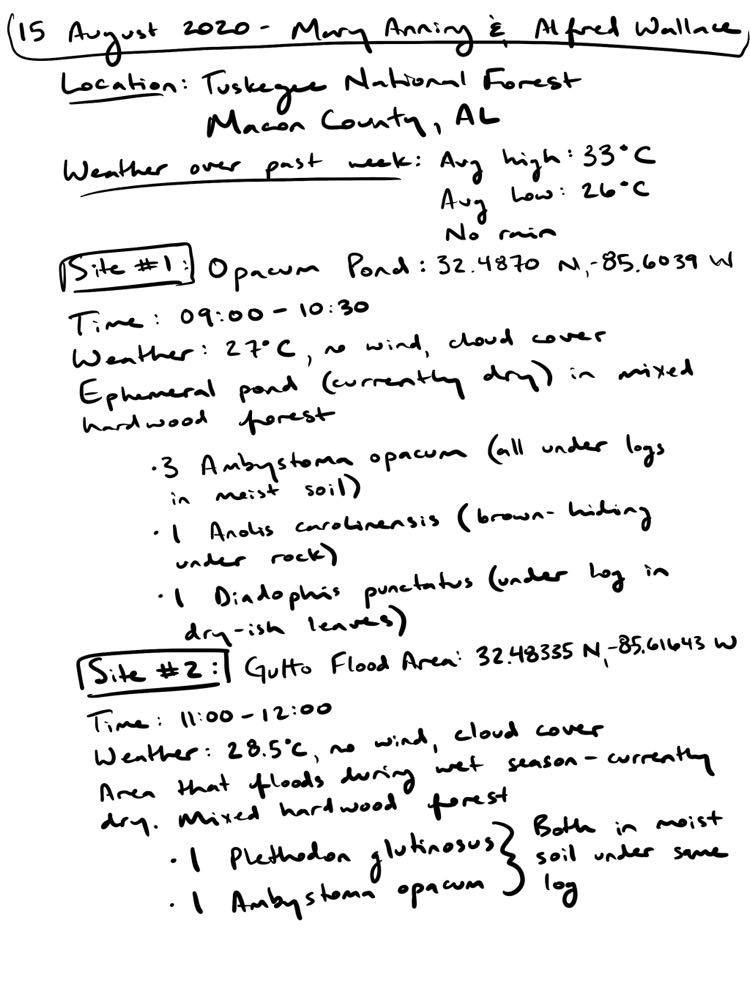
\includegraphics{FieldNoteExample.jpg}
  \label{fig:FieldNotes}
\end{figure}


\end{document}